\section{Exemplo motivador} % Seções são adicionadas para organizar sua apresentação em blocos discretos, todas as seções e subseções são automaticamente exibidas no índice como uma visão geral da apresentação, mas NÃO são exibidas como slides separados.

%----------------------------------------------------------------------------------------

\begin{frame}{Motivação: exemplo didático}
	
	Tomemos o exemplo motivador \cite{Chorin2013}.
	
	O sistema é constituído por duas partículas em 1 dimensão. Esse é um sistema de dois osciladores harmônicos sem interação acoplados, com o Hamiltoniano dado por:
	\begin{equation*}
		H = \frac{1}{2}\left(q_1^2 + q_2^2 + q_1^2 q_2^2 + p_1^2 + p_2^2\right)
	\end{equation*}
\end{frame}

\begin{frame}{Equações de movimento}
	O sistema é dado por:
	\begin{align*}
		\dot{q}_1 & = p_1,            \\
		\dot{p}_1 & = -q_1(1 + q_2^2) \\
		\dot{q}_2 & = p_2             \\
		\dot{p}_2 & = -q_2(1 + q_1^2) 
	\end{align*}
	
	\footnotesize{Onde $p_i$ e $q_i$ são o momento e a posição da partícula $i$}
	
	Temos que apenas $q_1(0)$ e $p_1(0)$ são conhecidos. E $q_2(0)$ e $p_2(0)$ são definidos por:
	\begin{equation*}
		W = \frac{e^{-H(q,p)}}{Z}
	\end{equation*}
	
\end{frame}

%--------------------------------------------------------

\begin{frame}{Simulação e estimativa}
	\begin{itemize}
		\item Para cada amostra de $q_2(0)$ e $p_2(0)$, obtemos uma nova trajetória de $q_1(t)$ e $p_1(t)$.
		\item Interesse em:
		      \begin{equation*}
		      	\mathbb{E}[q_1(t)\mid q_1(0), p_1(0)], \quad \mathbb{E}[p_1(t)\mid q_1(0), p_1(0)]
		      \end{equation*}
		\item Média feita sobre várias simulações.
	\end{itemize}
\end{frame}

%--------------------------------------------------------

\begin{frame}{Limitação da abordagem}
	\begin{itemize}
		\item A abordagem  é válida apenas para \textbf{tempos curtos}.
		\item Para $t$ grande: as médias se afastam dos valores reais.
	\end{itemize}
\end{frame}

%--------------------------------------------------------

\begin{frame}{Gráfico}
	\begin{figure}[h]
		\centering
		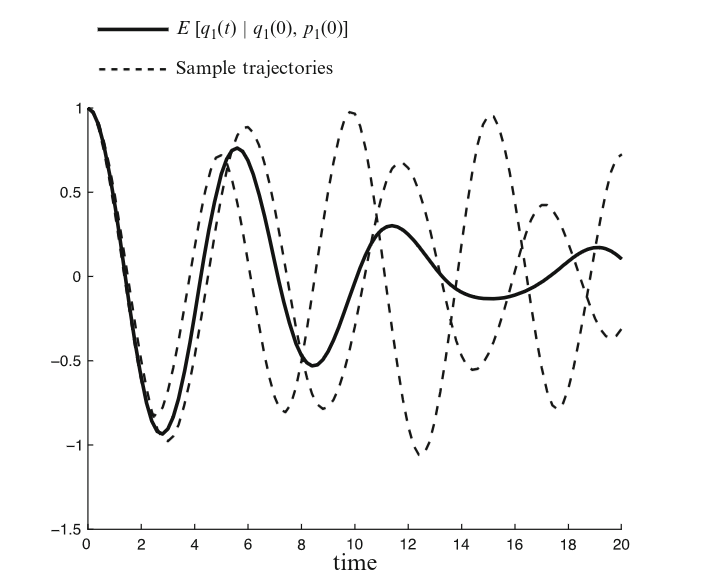
\includegraphics[width=0.4\textwidth]{03_SEMINARIO_MZ/02_APRESENTACAO/01_LATEX/img/grafico_motivacao.png}
		\caption{Simulação - Exemplo motivador}
		\label{fig:simulacao_exemplo_motivador}
	\end{figure}
\end{frame}
